\section{Introduction}
The remarkable progress of large language models (LLMs) in recent years has yielded substantial improvements in their reasoning capabilities. This progress is most evident in benchmarks involving complex mathematics \citep{cobbe2021training, hendrycks2021measuring} and coding tasks \citep{jain2024livecodebench, jimenez2023swe, chen2021evaluating, fan2023nphardeval}. Beyond these domains, researchers have also explored the logical reasoning abilities of LLMs from various angles, including propositional logic \citep{zhu2023dyval}, first-order logic \citep{han2022folio, parmar2024logicbench}, and propositional logic under different contexts \citep{hua2024disentangling}.


% why use the function classes as induction

% automatic evaluation
% controllable generation with controllable complexity
% dynamic generation

% other observation in experiment
% length changing: non systematic? 
% not enough, cannot find all rules
% o3: not minimum description

Despite significant progress in model capabilities, existing benchmarks predominantly focus on deductive reasoning, largely overlooking inductive reasoning. The former requires applying explicitly defined premises to derive valid conclusions, whereas the latter requires inferring the underlying principles, rules, or patterns from observations \citep{hawthorne2004inductive}. Both forms of reasoning are essential; inductive reasoning, in particular, is critical in domains such as scientific discovery where researchers seek to characterize natural laws based on empirical data \citep{grunwald2007minimum, hansen2001model} that captures complex phenomena. Figure~\ref{fig:demonstration} illustrates the differences between inductive and deductive reasoning.

\begin{wrapfigure}{r}{0.5\textwidth}
  \begin{center}
    \includegraphics[scale=0.35]{Fig/inductive_main.pdf}
    \vspace{-10pt}
    \caption{Deductive vs. Inductive Reasoning}
    \label{fig:demonstration}
  \end{center}
\end{wrapfigure}

In this paper, we address this gap by introducing \textbf{InductionBench}, a rigorous benchmark designed to assess LLMs' inductive reasoning abilities by testing whether they can infer a string-to-string transformation from a finite set of input–output pairs. A model must hypothesize the underlying relationship between inputs and outputs based on a finite set of examples and then extrapolate those rules to unseen strings. The process of discovering the underlying function from limited data reflects the core principles of inductive reasoning.

Our benchmark is grounded in the subregular hierarchy \citep{rogers2011aural, truthe2018hierarchy, graf2022diving, jager2012formal, heinz2018computational} (see Figure~\ref{fig:subregular}) for string-to-string mappings \citep{mohri1997finite}, focusing on input transformations restricted to regular functions. By systematically increasing task complexity across multiple classes in the subregular hierarchy, we gain detailed insights into how effectively LLMs detect, hypothesize, and generalize underlying rules from theoretically sufficient datapoints. 

We evaluate multiple state-of-the-art LLMs to understand LLM's inductive reasoning ability and identify factors that increase the difficulty of inductive reasoning tasks for LLMs, such as the length of the minimum-length description, the number of datapoints, and in-context examples. Through extensive experiments, we find that even advanced models such as o3-mini struggle with basic inductive tasks, highlighting a significant shortcoming in the current generation of LLMs. More detailed findings are presented in Section 5.

\begin{wrapfigure}{r}{0.5\textwidth}
    \centering
\resizebox{0.9\linewidth}{!}{
    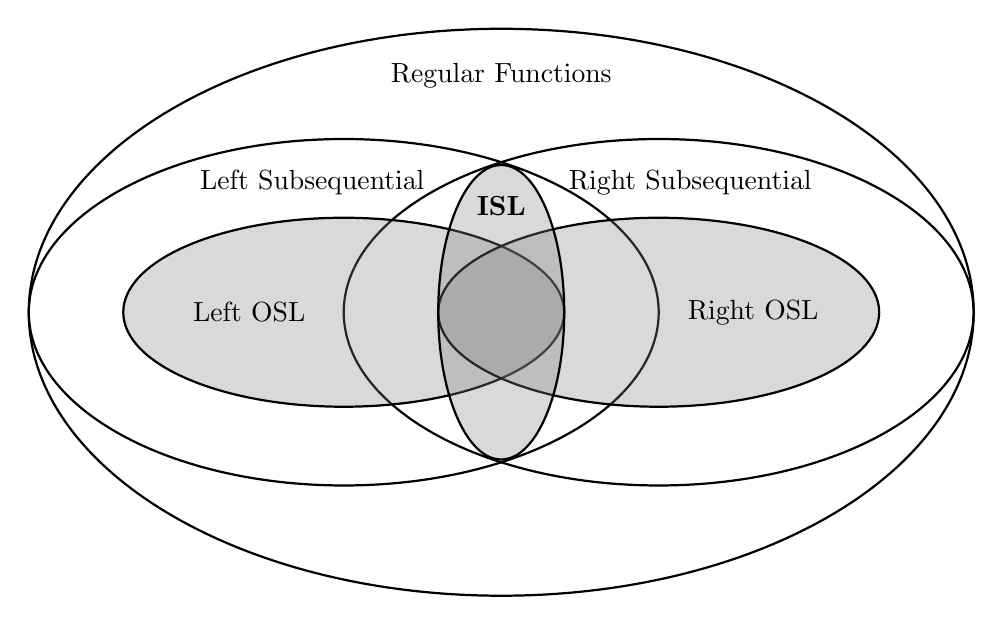
\begin{tikzpicture} %[font=\small]

  % 1. 大椭圆 Regular Functions
  \draw[thick, draw=black] 
       (0,0) ellipse (6 and 3.6);
  \node at (0,3) {Regular Functions};

  % 2. Left Subsequential
  \draw[
    thick, 
    draw=black, 
    fill=none, 
    fill opacity=0.3
  ] 
  (-2,0) ellipse (4 and 2.2);
  \node[] at (-2.4, 1.65) {Left Subsequential};

  % 3. Right Subsequential
  \draw[
    thick, 
    draw=black, 
    fill=none, 
    fill opacity=0.3
  ] 
  (2,0) ellipse (4 and 2.2);
  \node[] at (2.4, 1.65) {Right Subsequential};

  % 4. Left OSL
  \draw[
    thick, 
    % draw=red, 
    fill=gray, 
    fill opacity=0.3
  ] 
  (-2,0) ellipse (2.8 and 1.2);
  \node[] at (-3.2, 0) {Left OSL};

  % 5. Right OSL
  \draw[
    thick, 
    % draw=orange, 
    fill=gray,
    fill opacity=0.3
  ] 
  (2,0) ellipse (2.8 and 1.2);
  \node[] at (3.2, 0) {Right OSL};

  % 6. ISL (center overlap)
  \draw[
    thick, 
    % draw=purple,
    fill=gray, 
    fill opacity=0.3
  ] 
  (0,0) ellipse (0.8 and 1.87);
  \node[] at (0,1.35) {\textbf{ISL}};

\end{tikzpicture} }
    \caption{Subregular hierarchy in string-to-string maps}
    \vspace{-10pt}
    \label{fig:subregular}
\end{wrapfigure}